\section{Requirement Analysis}
This phase is crucial for developing a user-centered application like Expire Guard. It involves understanding the users' needs, goals, and tasks to ensure that Expire Guard's design and functionality align with their expectations and provide an optimal user experience.
\subsection{Competitor Analysis}
We have identified two main competitors that can be compared to Expire Guard. The first competitor is Google Calendar, a widely used application that allows users to create and manage events. Although it is not specifically designed to store and track document expiration dates, users can utilize it for this purpose by creating an event on the relevant date and time. Google Calendar's intuitive interface and integration with other Google services make it a versatile tool for managing schedules and reminders.\\
The second competitor is Evernote, a note-taking application that allows users to capture ideas, create to-do lists, and schedule memos. Evernote enables users to set alert triggers to notify them of their created memos, enhancing productivity and organization. While Evernote is primarily used for note-taking, its flexible tagging and search functionalities can be adapted for tracking document-related information, including expiration dates.\\
The following tables present a detailed comparison between Expire Guard and its competitors:\\
\begin{table}[H]
	
	\begin{tabularx}{\textwidth}{|X|X|X|}
		\hline
		\textbf{Element of Comparison} & \textbf{Expire Guard} & \textbf{Google Calendar} \\ 
		\hline
		\textbf{Audience} & Aimed at everyone with access to a smartphone and basic knowledge of it. & Aimed at everyone with access to a smartphone and basic knowledge of it. \\
		\hline
		\textbf{Document storage} & Users can store and organize all their important documents in a secure, cloud-based environment, ensuring easy access and management. & Difficult to distinguish between generic events and events related to documents. \\
		\hline
		\textbf{Document scan} & Users can add a scan of the document. & Not supported. \\
		\hline
		\textbf{Expiration Tracking} & Users can create a customized tracking system that reminds them of the expiration dates of documents with different alert periods, suiting their specific needs for different types of documents. & Users must manually decide the date on which to create an event to remind them of the expiration of a document. \\
		\hline
		\textbf{Communication with the Users} & Users are presented with an intuitive UI that guides them in the process of adding and tracking a document. & Simple calendar UI, easy to understand and well documented, simple event creation process. \\
		\hline
		\textbf{Feedback to the User} & When the User adds a new document tracking gets notified in the UI of the successful operation alongside an email. When an alert period is triggered, the User receives a notification on the smartphone and an email to their preferred email address. & When an event is added, the User receives an email to notify them of the new event. When the event approaches, the User is reminded of it with an email. \\
		\hline
		\textbf{Subscription} & Free unlimited features. & Free unlimited features. \\
		\hline
	\end{tabularx}
	\caption{Comparison between Expire Guard and Google Calendar}
\end{table}
\begin{table}[H]
	
	\begin{tabularx}{\textwidth}{|X|X|X|}
		\hline
		\textbf{Element of Comparison} & \textbf{Expire Guard} & \textbf{Evernote} \\
		\hline
		Audience  & Aimed at everyone with access to a smartphone and basic knowledge of it. & Aimed at young students with more than common tech and smartphone knowledge.
		
		\\
		\hline
		Document storage & Users can store and organize all their important documents in a secure, cloud-based environment, ensuring easy access and management. & Difficult to distinguish between generic memos and memos related to documents. \\
		\hline
		Document scan & Users can add a scan of the document & Users can add pictures alongside their memos \\
		\hline
		Expiration Tracking & Users can create a customized tracking system that reminds them of the expiration dates of documents with different alert periods, suiting their specific needs for different types of documents. & Users must manually decide the date in which they will be reminded of the memo about the document expiration. \\
		\hline
		Communication with the Users& Users are presented with an intuitive UI that guides them in to the process of adding and tracking a document. & More complex and structured UI, not so easy to understand but fairly intuitive, tracked, and well defined memo creation process. \\
		\hline
		Feeback to the User& When the User adds a new document and tracking gets notified in the UI of the successful operation alongside an email. When an alert period is triggered, the User receives a notify on the smartphone and an email con their preferred email address. & When a memo is added the User receives confirmation in the UI, when the memo reaches the alert period the User receives an email and a smartphone notify. \\
		\hline
		Subscription  & Free unlimited features. & Very limited free feature and multiple subscription tears to enhance them. \\
		\hline
	\end{tabularx}
	\caption{Comparison between Expire Guard and Evernote}
\end{table}
\noindent
Both comparisons demonstrate that our approach, focused on storing and tracking document expiration dates, is more effective in achieving the specific goal of notifying users about upcoming expirations based on their preferences. While Google Calendar and Evernote offer versatile functionalities, they cater to broader user needs beyond document expiration tracking. Our solution simplifies and enhances this process, making it more tailored and efficient compared to using Google Calendar or Evernote for this specific purpose.\\
\subsection{User Analysis}
The target users of this application are individuals with demanding jobs that require them to manage numerous document expiration dates, such as driver's licenses, legal documents, taxes, and more. The target profile is outlined as follows:
\begin{table}[H]
	\centering
	\begin{tabularx}{\textwidth}{XX}
		\textbf{AGE}& 18 - 50\\
		\textbf{GENDER}& Female/Male\\
		\textbf{REGION}& Europe Union\\
		\textbf{TECHNOLOGY}&Mobile applications/Smartphone\\
		\textbf{EDUCATION}& Any\\
	\end{tabularx}
\end{table}
\noindent
The next step is to define several personas and their corresponding scenarios. Personas are fictional characters created in user-centered design to embody the types of users who would have a genuine interest in using the application daily. They serve a pivotal role in uncovering insights about the audience, particularly representative of working professionals in the European Union.\\
Once personas are established, defining user scenarios becomes essential for a deeper understanding of each user's needs. These scenarios are narrative stories crafted to analyze how users would interact with and benefit from the application in various situations.\\
In the following subsection, three distinct personas will be presented, accompanied by a scenario for each. These scenarios are instrumental in advancing user analysis and informing the application's development process.\\
\subsubsection{First persona: David}

\begin{minipage}[t]{0.3\textwidth} % Adjust the width as needed
	\vspace{0pt} % Adjust vertical position if needed
	\centering
	\vspace{0pt}
	
\includegraphics[width=\textwidth]{../Draw.io diagrams/alex.jpeg}
\end{minipage}%
\hfill
\begin{minipage}[t]{0.65\textwidth} % Adjust the width as needed
	\paragraph{Persona:\newline}
	\vspace{0pt} % Adjust vertical position if needed
	\noindent
	\vbox{
	 \vspace{5pt}
	 David, a 35-year-old real estate agent, starts his day early in the real estate office. His desk is cluttered with property listings, lease agreements, and maintenance records. David prides himself on providing excellent service to landlords and tenants alike, but he often finds himself overwhelmed by the sheer volume of documents and deadlines he needs to manage.
	}
	\paragraph{Scenario:\\}
	\vspace{0pt} % Adjust vertical position if needed
	\noindent
	\vbox{
	 \vspace{5pt}
	 David prepares for a morning meeting with a potential landlord client, he notices a lease agreement buried beneath a stack of papers. It's a renewal notice for a rental property due in two weeks. David recalls an incident where he missed a lease renewal deadline, causing frustration for the tenant and a delay in securing rental income for the landlord. He realizes that managing multiple property leases and maintenance schedules manually is becoming increasingly challenging and prone to errors.
	}
\end{minipage}

\subsubsection{Second persona: Emily}

\begin{minipage}[t]{0.65\textwidth} % Adjust the width as needed
	\paragraph{Persona:\\}
	\vspace{0pt} % Adjust vertical position if needed
	\noindent
	\vbox{
		\vspace{5pt}
		Emily, a 33-year-old, is a freelancer working from her home office. Her clients are scattered across the globe, demanding high-quality designs and timely deliveries. Emily juggles multiple projects, each with its own set of contracts and deadlines. Additionally, she relies on various software tools, all of which require periodic license renewals. She also needs to keep track of personal documents like her passport and ID, as she frequently travels for work.
	}
	\paragraph{Scenario:\\}
	\vspace{0pt} % Adjust vertical position if needed
	\noindent
	\vbox{
		\vspace{5pt}
		One Tuesday afternoon, Emily is deep into designing a new logo for a major client when her design software suddenly stops working. After a few moments of confusion, she realizes her software license has expired. This unexpected disruption causes her to miss an important client meeting, leading to frustration and stress. Determined to prevent such incidents in the future, Emily searches for a comprehensive solution.
	}
\end{minipage}
\hfill
\begin{minipage}[t]{0.3\textwidth} % Adjust the width as needed
	\vspace{0pt} % Adjust vertical position if needed
	\centering
	\vspace{0pt}
	
\includegraphics[width=\textwidth]{../Draw.io diagrams/emily.jpeg}
\end{minipage}%
\clearpage
\subsubsection{Third persona: Alex}

\begin{minipage}[t]{0.3\textwidth} % Adjust the width as needed
	\vspace{0pt} % Adjust vertical position if needed
	\centering
	\vspace{0pt}
	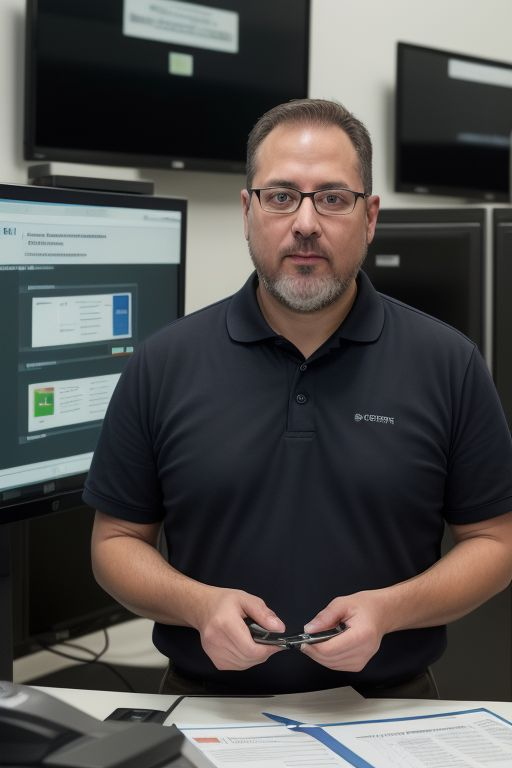
\includegraphics[width=\textwidth]{../Draw.io diagrams/david.jpeg}
\end{minipage}%
\hfill
\begin{minipage}[t]{0.65\textwidth} % Adjust the width as needed
	\paragraph{Persona:\\}
	\vspace{0pt} % Adjust vertical position if needed
	\noindent
	\vbox{
		\vspace{5pt}
		Alex a 45-year-old small business owner, runs a local hardware store. Alex is responsible for every aspect of the business, from inventory management to customer service. One of his most critical yet challenging tasks is managing various business-related documents, such as licenses, permits, and insurance policies. With a busy schedule and numerous responsibilities, Alex often struggles to keep track of expiration dates, leading to potential legal and operational issues.
	}
	\paragraph{Scenario:\\}
	\vspace{0pt} % Adjust vertical position if needed
	\noindent
	\vbox{
		\vspace{5pt}
		One day, while preparing for a busy weekend at the store, Alex receives a notice that his business license is about to expire. He realizes that he had forgotten to renew it. This oversight could result in fines or even temporary closure, which would be detrimental to his business. Determined to find a solution, Alex searches for a reliable way to manage his documents.
	}
\end{minipage}
